\documentclass[modern]{aastex62}

\usepackage{color}
\usepackage{amsmath}
\usepackage{enumitem}
\usepackage{graphicx}
\usepackage{mathrsfs}


\definecolor{bcolor}{RGB}{0, 51, 153}
\definecolor{gcolor}{RGB}{51, 153, 51}
\hypersetup{linkcolor=bcolor,citecolor=bcolor,filecolor=cyan,urlcolor=bcolor}

\newcommand{\vdag}{(v)^\dagger}
\newcommand\aastex{AAS\TeX}
\newcommand\latex{La\TeX}

\received{\color{red} MM/DD/YY}
\revised{\color{red} MM/DD/YY}
\accepted{\color{red} MM/DD/YY}
\submitjournal{\color{red} JOURNAL}

\shorttitle{Birky et al.}
\shortauthors{Birky et al.}


\begin{document}

\title{DATA DRIVEN MODELS FOR APOGEE M DWARFS}


\correspondingauthor{Jessica Birky}
\email{jbirky@ucsd.edu}

\author[0000-0002-7961-6881]{Jessica Birky}
\affil{Center for Astrophysics and Space Science, University of California San Diego, La Jolla, CA 92093, USA}
\affil{Max-Planck-Institut f\"ur Astronomie, K\"onigstuhl 17, D-69117 Heidelberg, Germany}

\author[0000-0003-2866-9403]{David W. Hogg}
\affil{Max-Planck-Institut f\"ur Astronomie, K\"onigstuhl 17, D-69117 Heidelberg, Germany}
\affiliation{Center for Computational Astrophysics, Flatiron Institute, 162 Fifth Ave, New York, NY 10010, USA}
\affiliation{Center for Cosmology and Particle Physics, Department of Physics, New York University, 726
Broadway, New York, NY 10003, USA}
\affil{Center for Data Science, New York University, 60 Fifth Ave, New York, NY 10011, USA}

\author[0000-0003-3654-1602]{Andrew Mann}
\affil{Department of Astronomy, Columbia University, 550 West 120th Street, New York, NY 10027, USA}

\author[0000-0002-6523-9536]{Adam Burgasser}
\affil{Center for Astrophysics and Space Science, University of California San Diego, La Jolla, CA 92093, USA}

\begin{abstract}

The Cannon \citep{Ness:2015} is a flexible, data-driven spectral modeling and parameter inference framework, demonstrated on high-resolution Apache Point Galactic Evolution Experiment (APOGEE; $\lambda/\Delta\lambda\sim22,500$, $1.5-1.7 \mu m$) spectra of giant stars to estimate stellar labels (T$_{\rm eff}$, logg, [Fe/H], and chemical abundances) to precisions higher than the model-grid pipeline. The lack of reliable stellar parameters reported by the APOGEE pipeline for temperatures less than $\sim3550K$ \citep{Schmidt:2016}, motivates the extension of this approach to M dwarf stars. Using a training set of 51 M dwarfs with spectral types ranging M0-M9 obtained from SDSS optical spectra, we demonstrate that The Cannon can infer spectral types to a precision of 0.6 types. We then use 30 M dwarfs ranging $3072 < T_{\rm eff} < 4131K$, and -0.48 $<$ [Fe/H] $<$ 0.49 to train a two-parameter model precise to 44K and 0.05 dex respectively. Finally we compare our temperature/metallicty model to theoretical models of M dwarf atmospheres (PHOENIX, \citealt{Husser:2013}; BTSETTL, \citealt{Allard:2011}) and identify features of missing line strengths.

\end{abstract}

\keywords{stars: Mdwarfs -- stellar parameters}
 
%%==========================================================================================
\section{Introduction} \label{sec:intro}

% \begin{enumerate}
Very low mass (VLM) stars are the most abundant type of star, comprising $\sim 70 \%$ of the galaxy's population by number \citep{Bochanski:2010} and $\sim 40 \%$ by mass are known to have lifespans longer than the age of the universe (billions or up to trillions of years) \citep{Laughlin:1997} making them an interesting probe of Milky way populations \citep{Bochanski:2007}.


%define 'labels' - could be physical parameters or more empirical 

\begin{enumerate}

\item[-] Define what parameters/classifications are important for Mdwarfs. We want to estimate physical parameters (such as Teff, logg, metallicity) and empirical parameters/classifications (SPT, etc.), which we will refer to as \emph{stellar labels}.

\item[-] Various attempts / samples for which people have tried to make substantial catalogs of M-dwarfs with physical labels on them (\citealt{West:2011} is the largest M dwarf catalog of $\sim$ 70k sources... Terrien, Mann, Newton, Dressing catalogs) 

\item[-] brief importance statment about APOGEE - new instrumentation has allowed for new opportunity - high resolution and large datasets of Mdwarfs are now available

\item[-] Describe M dwarf studies that have already been conducted in APOGEE (\citealt{Schmidt:2016} -- analyzed trends and reliablility of ASPCAP parameters for K/M dwarfs; \citealt{Souto:2017} -- modeled 2 M dwarfs, determined Teff/logg/metallicity + 13 elemental abundances; \citealt{Desphande:2013} -- modeled rotational and radial velocites for several hundred M dwarfs; \citealt{Rajpurohit:2018} -- tested BTSettl model grids on 45 M dwarfs, estimated Teff/logg/metallicity). \citealt{Gilhool:2018}; \citealt{Skinner:2018}.

\item[-] Why is there a problem labeling M dwarfs (and especially for high res APOGEE spectra)? Emphasize issues: models dont accurately reproduce data; empirical standards are relative not absolute. 

 (1) model the spectra using atmospheric models (BTSettl, \citealt{Allard:2011}; PHOENIX, \citealt{Husser:2013}, MARCS \citealt{Gustafsson:2008}, ATLAS \citealt{Castelli:2004}, etc.) find some places in literature where people have tried these on M dwarfs (\citealt{Rajpurohit:2014}, \citealt{Rajpurohit:2018}) - however missing opacities, and complexities due to molecules/clouds/chemistry make this difficult (\citealt{Allard:2013})--models don't accurately reproduce spectra plus unquantified systematic errors; 

 (2) model narrow wavelegth region where models are good, look at specific features (\citealt{Rojas-Ayala:2012}...), or reduce resolution (\citealt{Casagrande:2008} estimated effective temperatures, bolometric luminosities, and metallicities using optical and infrared photometries) -- however we want to use \emph{all} of the data!

 (3) using empirical classifications/templates/standards - SPT, luminosity class - this is a relative system but does not provide an absolute standard for measuring physical parameters

\item[-] Why The Cannon approach? brief importance statment cannon and what it does (cite \citealt{Ness:2015}, \citealt{Ho:2017a}, \citealt{Casey:2016})

 (1) Can be used to amplify a small number of labeled M-dwarfs in a training set into a huge number of labeled M-dwarfs, provided that there are overlapping objects; 

 (2) Make the point that The Cannon does not require us to have good M-dwarf models in the APOGEE wavelength range at all 

 (3) better than template matching in that it is using less sparsely sampled known mdwarfs

\end{enumerate}

%photometric data, HR digram, comparison to evolutionary models


%%==========================================================================================
\section{Data} \label{sec:data}

\subsection{APOGEE Survey}
% \begin{enumerate}
% \item[-] Describe the APOGEE data (survey mission: \citealt{Majewski:2015}; target selection: \citealt{Zasowski:2013}; ASPCAP pipeline: \citealt{Perez:2016}). 

% \item[-] Some M dwarfs in APOGEE proposed as ancilliary targets (Blake/Covey sources), plus an unknown number observed unintentionally \citep{Desphande:2013}.
% \end{enumerate}

The APOGEE survey \citep{Majewski:2015} of the Sloan Digital Sky Survey III (SDSS-III; \citealt{Eisenstein:2011}) is a high resolution (R$\sim$22,500), H-band (1.5-1.7$\mu$m) survey which has observed over 260,000 stellar spectra since its fourteenth data release (DR14; \citealt{Abolfathi:2017}). Fundamental parameters for each of these stars are estimated by the APOGEE Stellar Parameter and Chemical Abundances Pipeline (ASPCAP; \citealt{Perez:2016}), which employs a $\chi^2$ fitting procedure using the FERRE code to fit ATLAS9 radiative transfer models \citep{Castelli:2004} to determine atmospheric parameters, 15 chemical abundances and micro-turbulence parameters (T$_{\rm eff}$, log g, [Fe/H], [$\alpha$/M], [C/M], [N/M]; \citealt{Meszaros:2012}). 

APOGEE is primarily targeted for bright stellar populations, with de-reddened photometry and color cutoffs of $7 \leq H \leq 13.8$ and $[J-K]_0 \geq 0.5$ \citep{Zasowski:2013} with the objective of studying galactic composition and evolution. However numerous cool, main sequence sources have also been observed either accidentally, or as targets proposed by the M dwarf ancilliary survey \citep{Desphande:2013} (specific estimate based on Gaia?).


\subsection{Training Samples}

The Cannon is a \emph{generative model} which parameterizes the flux at each pixel of a spectrum in terms of a set of stellar labels (a flexible number of parameters chosen by the user; described in more detail in Section \ref{sec:cannon}). The model in this sense is used to \emph{transfer} labels from spectra which we know parameters for to those which we do not. Hence this data-driven approach effectively removes the challenges of physically modeling the atmosphere of a star (and common issues associated such as incomplete line lists or opacities), provided that we have a subset of spectra in the dataset with known (ideally very accurately measured) \emph{reference labels} that can be measured from other surveys/methods that are easier to infer from. 

For the purpose of this study we have constructed two different training samples: first a one-dimensional \emph{spectral type model}, and second a two-dimensional \emph{physical parameter model} which describes the temperature and metallicity. The choice of training labels, dimensionality of our data set, and requirements for a good training set we discuss further in Section \ref{sec:discussion}.

The spectral type sample consists of 51 sources, spanning M0-M9 cross-matched from the \citealt{West:2011} (hereafter W11) catalog of 78,841 M dwarfs from SDSS. For each source in the catalog, spectral types were determined both through an automated routine using The Hammer \citep{Covey:2007} and by visual inspection to a reported accuracy of $\pm$1 type.

The physical parameter sample consists of 30 sources with reference labels distributed over $3072 < T_{\rm eff} < 4131K$, and -0.48 $<$ [Fe/H] $<$ 0.49 drawn from \citealt{Mann:2015} (hereafter M15). The M15 catalog in total contains 183 sources selected from CONCH-SHELL \citep{Gaidos:2013} and with infrared spectra taken in follow up from the SpeX Spectograph. Effective temperatures are measured by comparison of BT-SETTL atmospheric models \citep{Allard:2011} to optical spectra. A subsample of 29 sources with measured angular diameters and bolometric fluxes from long-baseline optical interferometry are used to callibrate effective temperature measurements. Relative uncertainty from the callibration sample is measured to be \color{red}{$\sim$30K (check this)}\color{black}, which added in quadrature to the scatter from model comparison gives a total reported uncertainty of $\sim$60K in T$_{\rm eff}$. 


Spectral types reported by M15 for the sources using optical molecular band indices (by the method of \citealt{Lepine:2013}) and ranged K7.3--M4.9 for the subsample we used, although these labels were not included in the model training.

We note that surface gravity (logg) and rotational velocity (vsini) parameters are not included as training labels because...

% \begin{figure}[ht]
% \plottwo{figures/west_train_dist.png}{figures/mann_train_dist.png}
% \caption{Spectral type model: training label vs. test label.} \label{fig:west_selftest} \label{fig:train_dist}
% \end{figure}

\subsection{Data Processing}

We use the aspcapStar spectra (see \citealt{Perez:2016} for a complete description of the pipeline).

APOGEE data products come in several types of files: ap1D, apVisit, apStar, and aspcapStar. SNR of stars in our sample .

Describe ASPCAP spectra files and Ness continuum normalization procedure.


%%==========================================================================================
\section{Methods} \label{sec:cannon}

\subsection{The Cannon: A Data-Driven Approach}

\begin{enumerate}
\item[-] Describe the assumptions of the model: (1) Sources with identical labels have near-identical flux at each pixel; (2) Expected flux at each pixel varies continuosly with change in label. 
\item[-] Briefly describe modeling procedure (training step, test step, quadratic labels, etc.), refer to \citealt{Ness:2015} for full description.
\item[-] Briefly describe model inputs and outputs (1D spectral type model and 2D teff/metallicity and label vectors for those). Mention other models we've tested.
\end{enumerate}

Constructing such a model requires two steps: first the \emph{training step} in which the generative model is constructed at each pixel from the set of reference labels and fluxes, and second the \emph{test step} in which the model is applied to determine the labels of a spectrum 

% The key advantages of The Cannon being:
% Data-driven models take away the challenge of directly infering labels from a survey, instead we \emph{transfer labels} from another survery that is more accurate or easier to model.

Following from the procedure of \citealt{Ness:2015} and \citealt{Ho:2017a} we adopt a model that assumes the flux at each pixel of the spectrum is parameterized as a function \textit{g} 
\begin{equation}
	f_{n\lambda} = g(\ell_n | \theta_{\lambda}) + {\rm noise}
\end{equation}

\begin{equation}
	f_{n\lambda} = \theta_{\lambda}^{T} \cdot \ell_{n} + [s_{\lambda}^{2} + \sigma_{n\lambda}^{2}] \,\xi_{n\lambda}
\end{equation}

Quadratic label vectors:
\begin{equation}
	\ell_{n} = [1, SPT, SPT^{2}]
\end{equation}

\begin{equation}
	\ell_{n} = [1, T_{\rm eff}, [Fe/H], T_{\rm eff} \cdot [Fe/H], [Fe/H]^{2}]
\end{equation}


%%==========================================================================================
\section{Experimental Results} \label{sec:results}

\subsection{Spectral Type Model}

\begin{enumerate}
\item[-] We trained The Cannon on 51 M dwarfs with a one-dimensional spectral type label, and obtained a precision of $\pm$0.8 spectral types, more precise than the original training label uncertainty of $\pm$1 spectral type.
\item[-] Two tests of consistency were used to assess the validity of our derived test labels: Figure \ref{fig:west_selftest} displays the label self-test for the spectral type model, and Figure  displays 
\end{enumerate}


\begin{enumerate}
\item[-] For the physical parameter model we trained The Cannon on 30 M dwarfs with a two-dimensional with temperature/metallicity labels, and was able to achieve precisions of 44K/0.05dex respectively, more precise than both of the original training label uncertainties of 60K/0.08dex.

\item[-] Two tests of consistency were used to assess the validity of our derived test labels: Figure \ref{fig:west_selftest} displays the label self-test for the spectral type model, and Figure 2 displays 

\item[-] Vsini and logg were not included as training parameters. Vsini is less import of a parameter as the sample consists of mainly old, slowly rotating sources (check what are ages?). Logg because?
\end{enumerate}

\begin{enumerate}
\item[-] Describe derivative plots and jacknife error estimation.
\end{enumerate}


%%==========================================================================================
\section{Discussion} \label{sec:discussion}

\begin{enumerate}
\item[-] Brief summary of what we did and found

\item[-] Things we learned along the way: For example, not all training sets worked well in our experiments, probably because they were too small or had too little dynamic range.

\item[-] \color{gcolor}{HOGG: Some discussion of precision and accuracy: The Cannon can produce precise results, but is only as accurate as its training set.}\color{black}

\item[-] Some discussion of whether the derivatives are sensible or surprising. \color{red}{Add derivative plots.}\color{black}

\item[-] The Cannon as a test of evaluating training parameter accuracy? 
\end{enumerate}

%%==========================================================================================
\acknowledgements
We would like to acknowledge Derek Homeier (Universit{\"a}t Heidelberg), Wolfgang Bradner (MPIA), Hans Walter Rix (MPIA), Anna-Christina Eilers (MPIA), Anna Ho (Caltech), and Jackie Faherty (AMNH) for constructive discussions in the process of this project, as well as Bertrand Goldman (MPIA) and those who have supported the internship program at the Max Planck Institute f{\"u}r Astronomie for providing JB with funding and hospitality. \color{red}Software: The Cannon, numpy, matplotlib... \color{black}

\color{gcolor}{HOGG: SDSS acknowledgments... Grants and stuff...}\color{black}  

%%==========================================================================================
%% Figures

\begin{figure}[ht]
\begin{center}
\includegraphics[width=16cm]{figures/west_self_test_spt.png}
\end{center}
\caption{Spectral type model: training label vs. test label.} \label{fig:west_selftest}
\end{figure}

\subsection{Temperature/Metallicity Model}
\begin{figure}[ht]
\begin{center}
\includegraphics[width=16cm]{figures/self_and_validation_test_teff.png}
\includegraphics[width=16cm]{figures/self_and_validation_test_fe_h.png}
\end{center}
\caption{Temperature and Metallicity label self test.} \label{fig:mann_selftest}
\end{figure}


\begin{figure}[ht]
\plotone{figures/1_Spectral_Sequence.pdf}
\plotone{figures/2_Spectral_Sequence.pdf}
\plotone{figures/3_Spectral_Sequence.pdf}
\caption{ Spectral sequence of dwarfs in training set M0-M9; chip 1 of APOGEE
spectrum with highlighted spectral type sensitive regions identified in \citealt{Desphande:2013}.} \label{fig:sp_sequence}
\end{figure}

\begin{figure}[ht]
\begin{center}
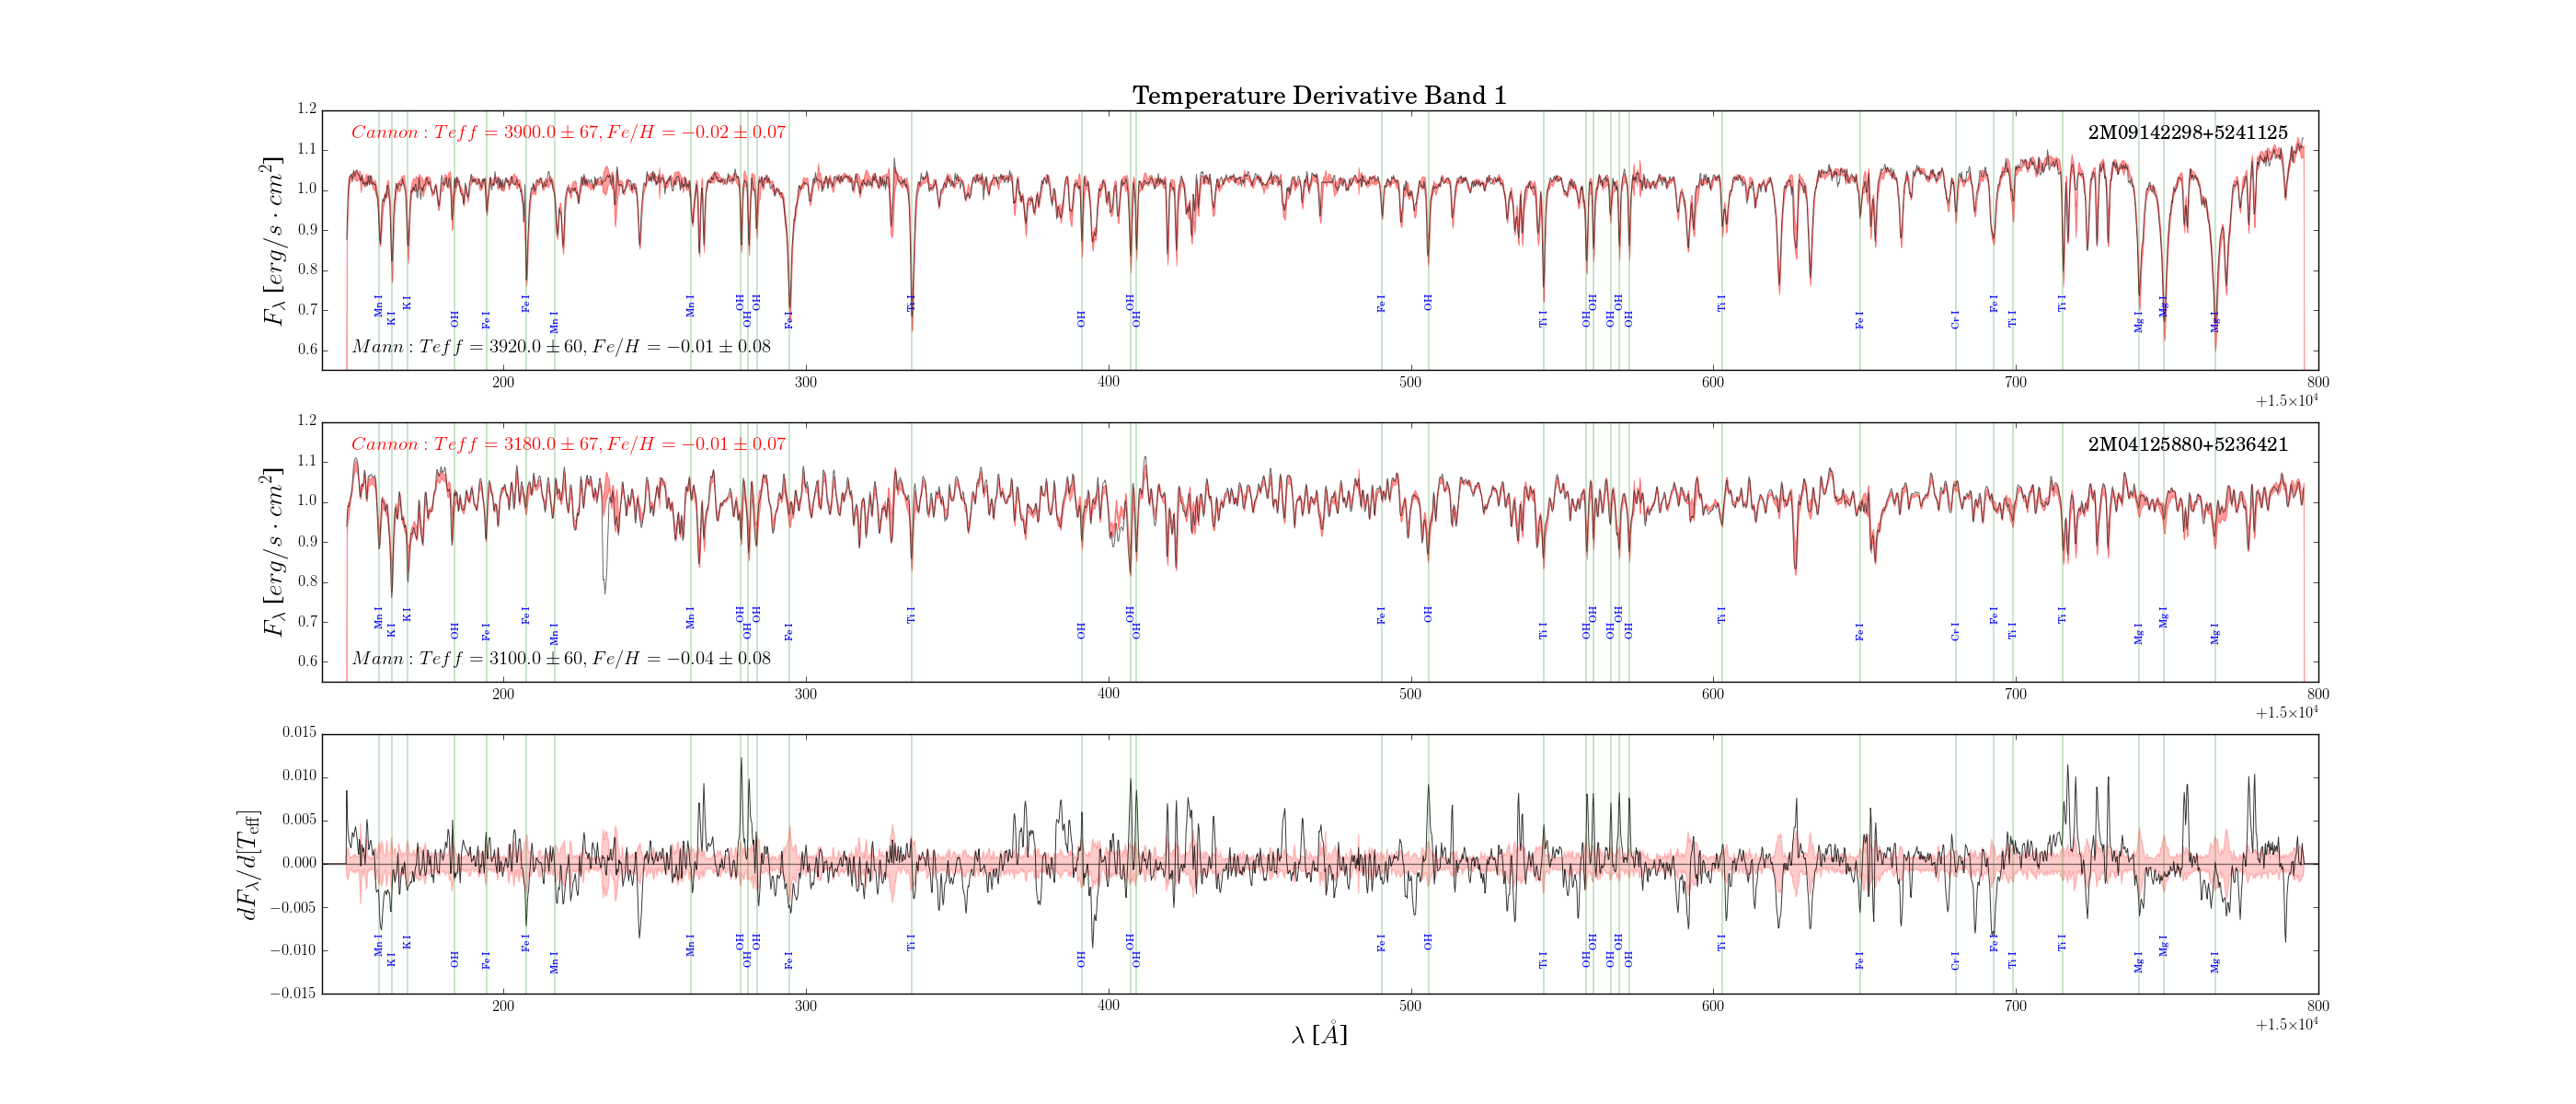
\includegraphics[width=16cm]{figures/demo_derivatives_teff1.png}
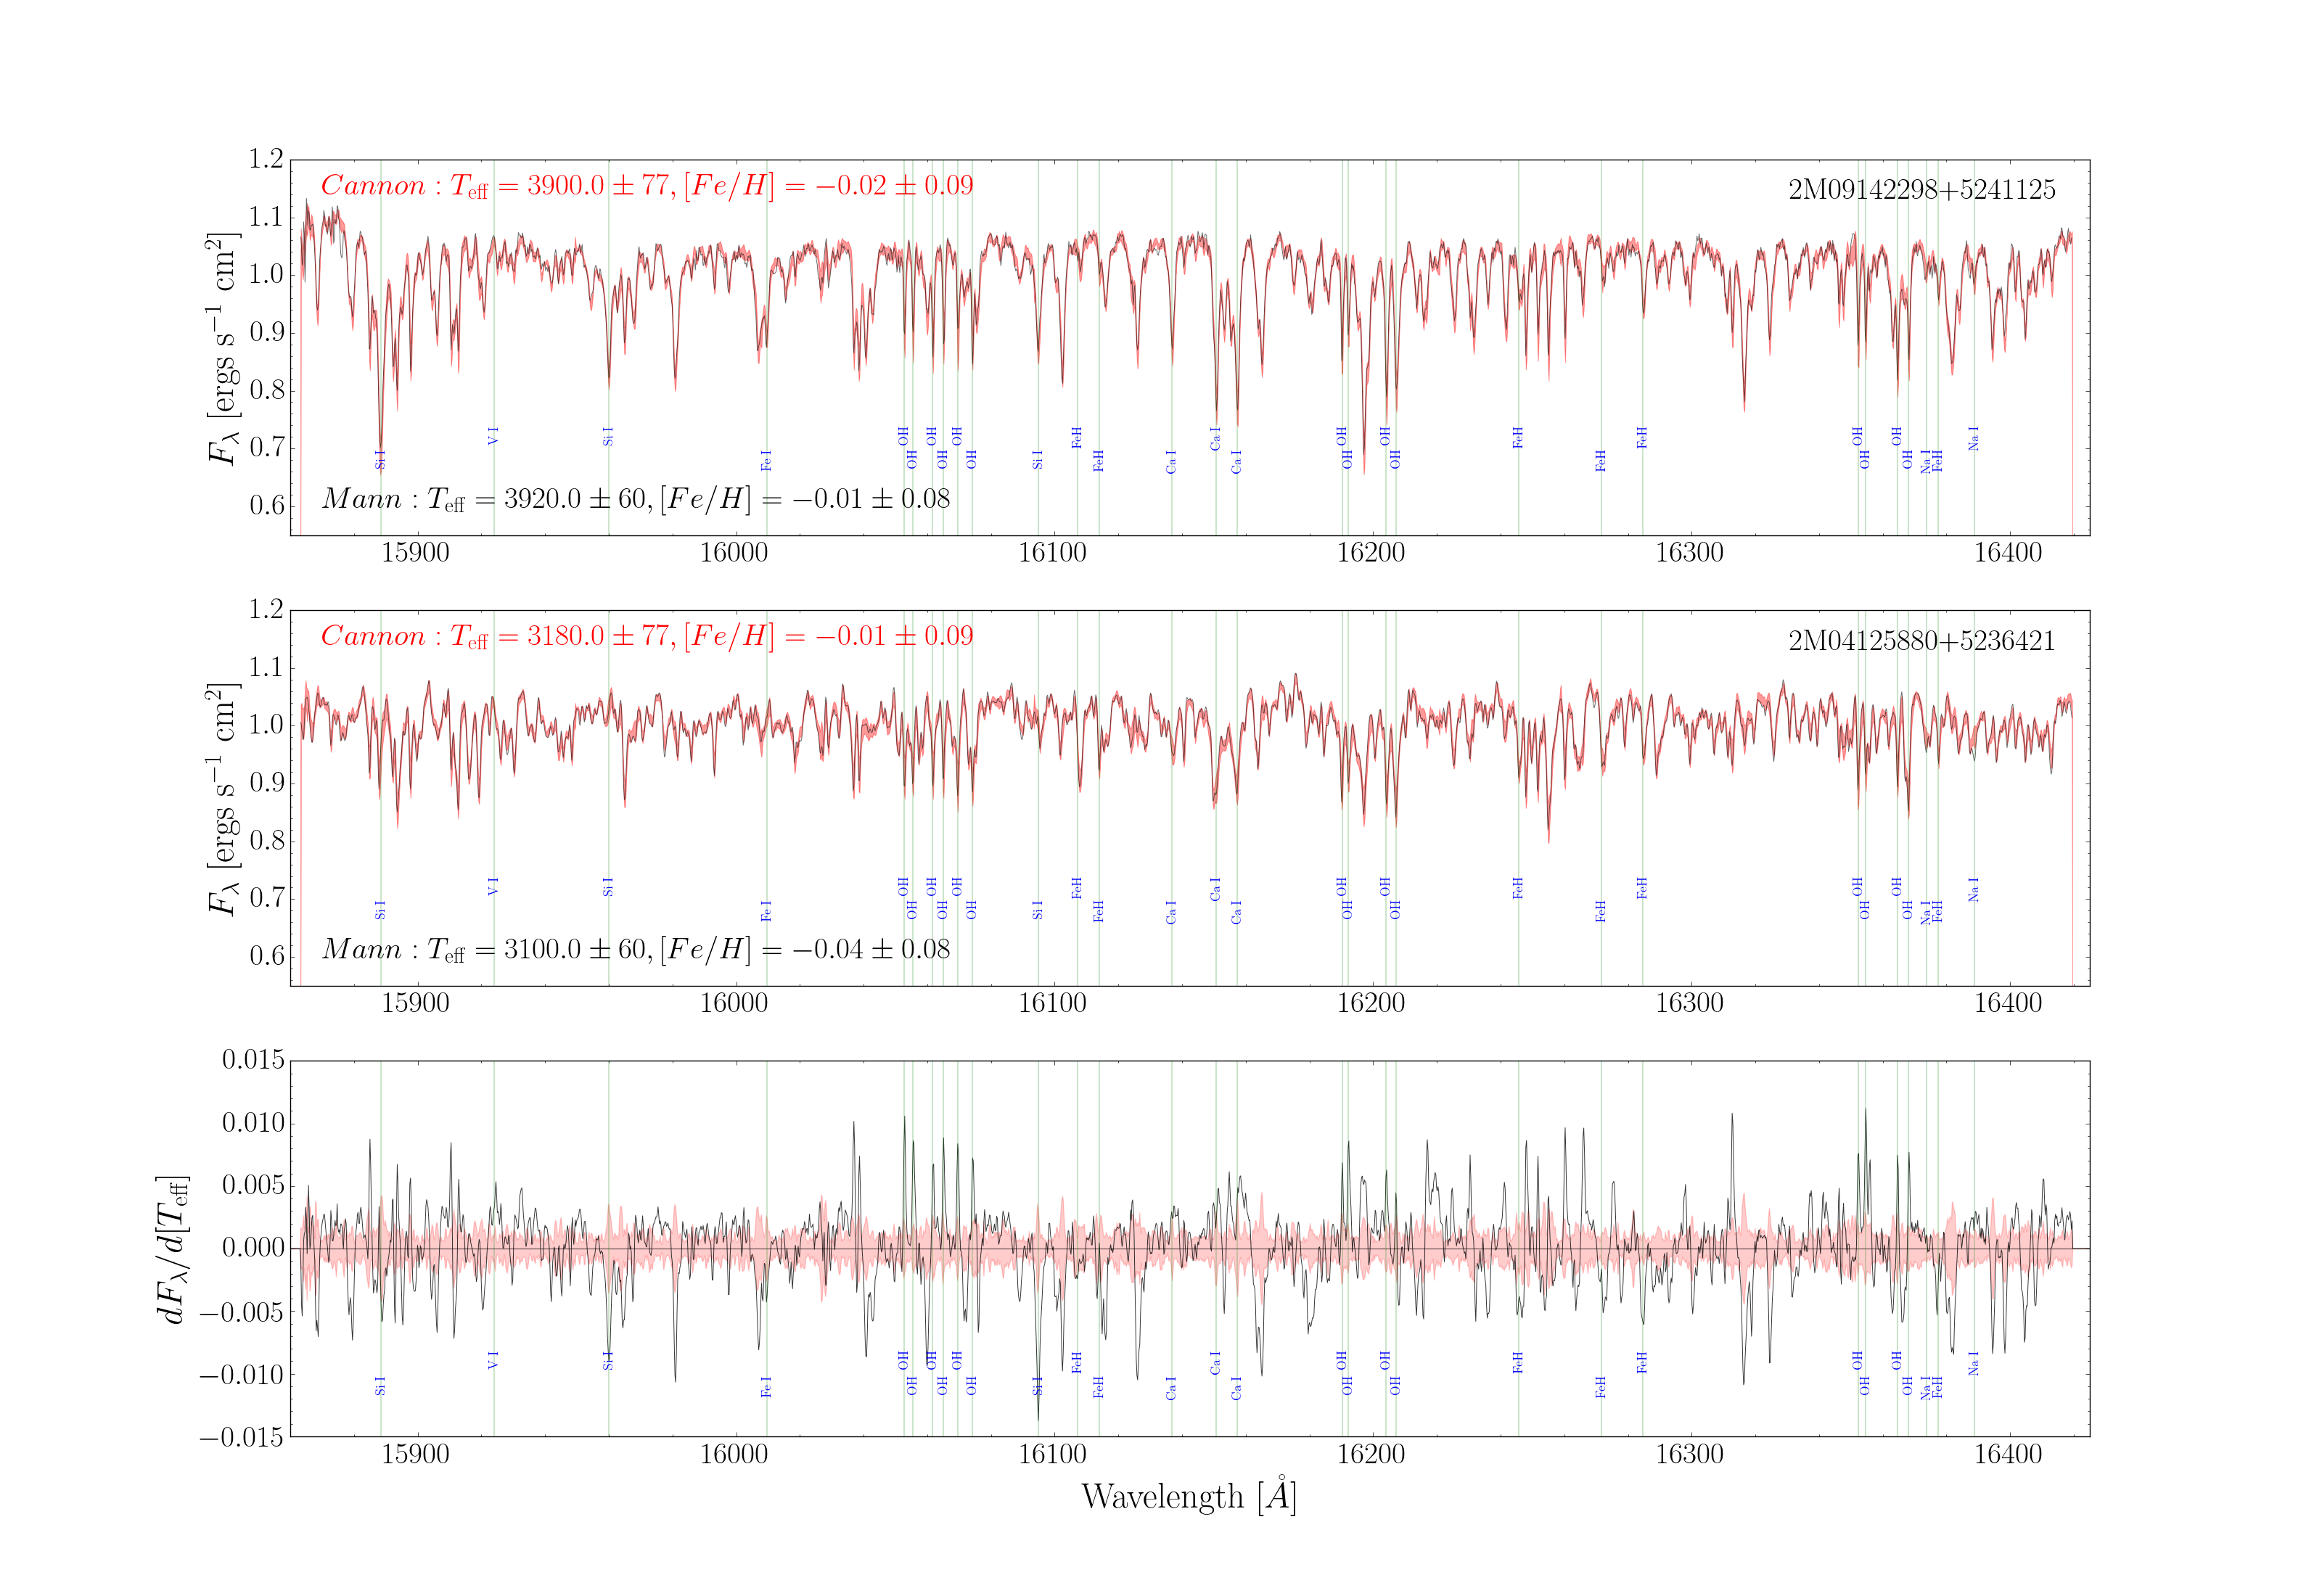
\includegraphics[width=16cm]{figures/demo_derivatives_teff2.png}
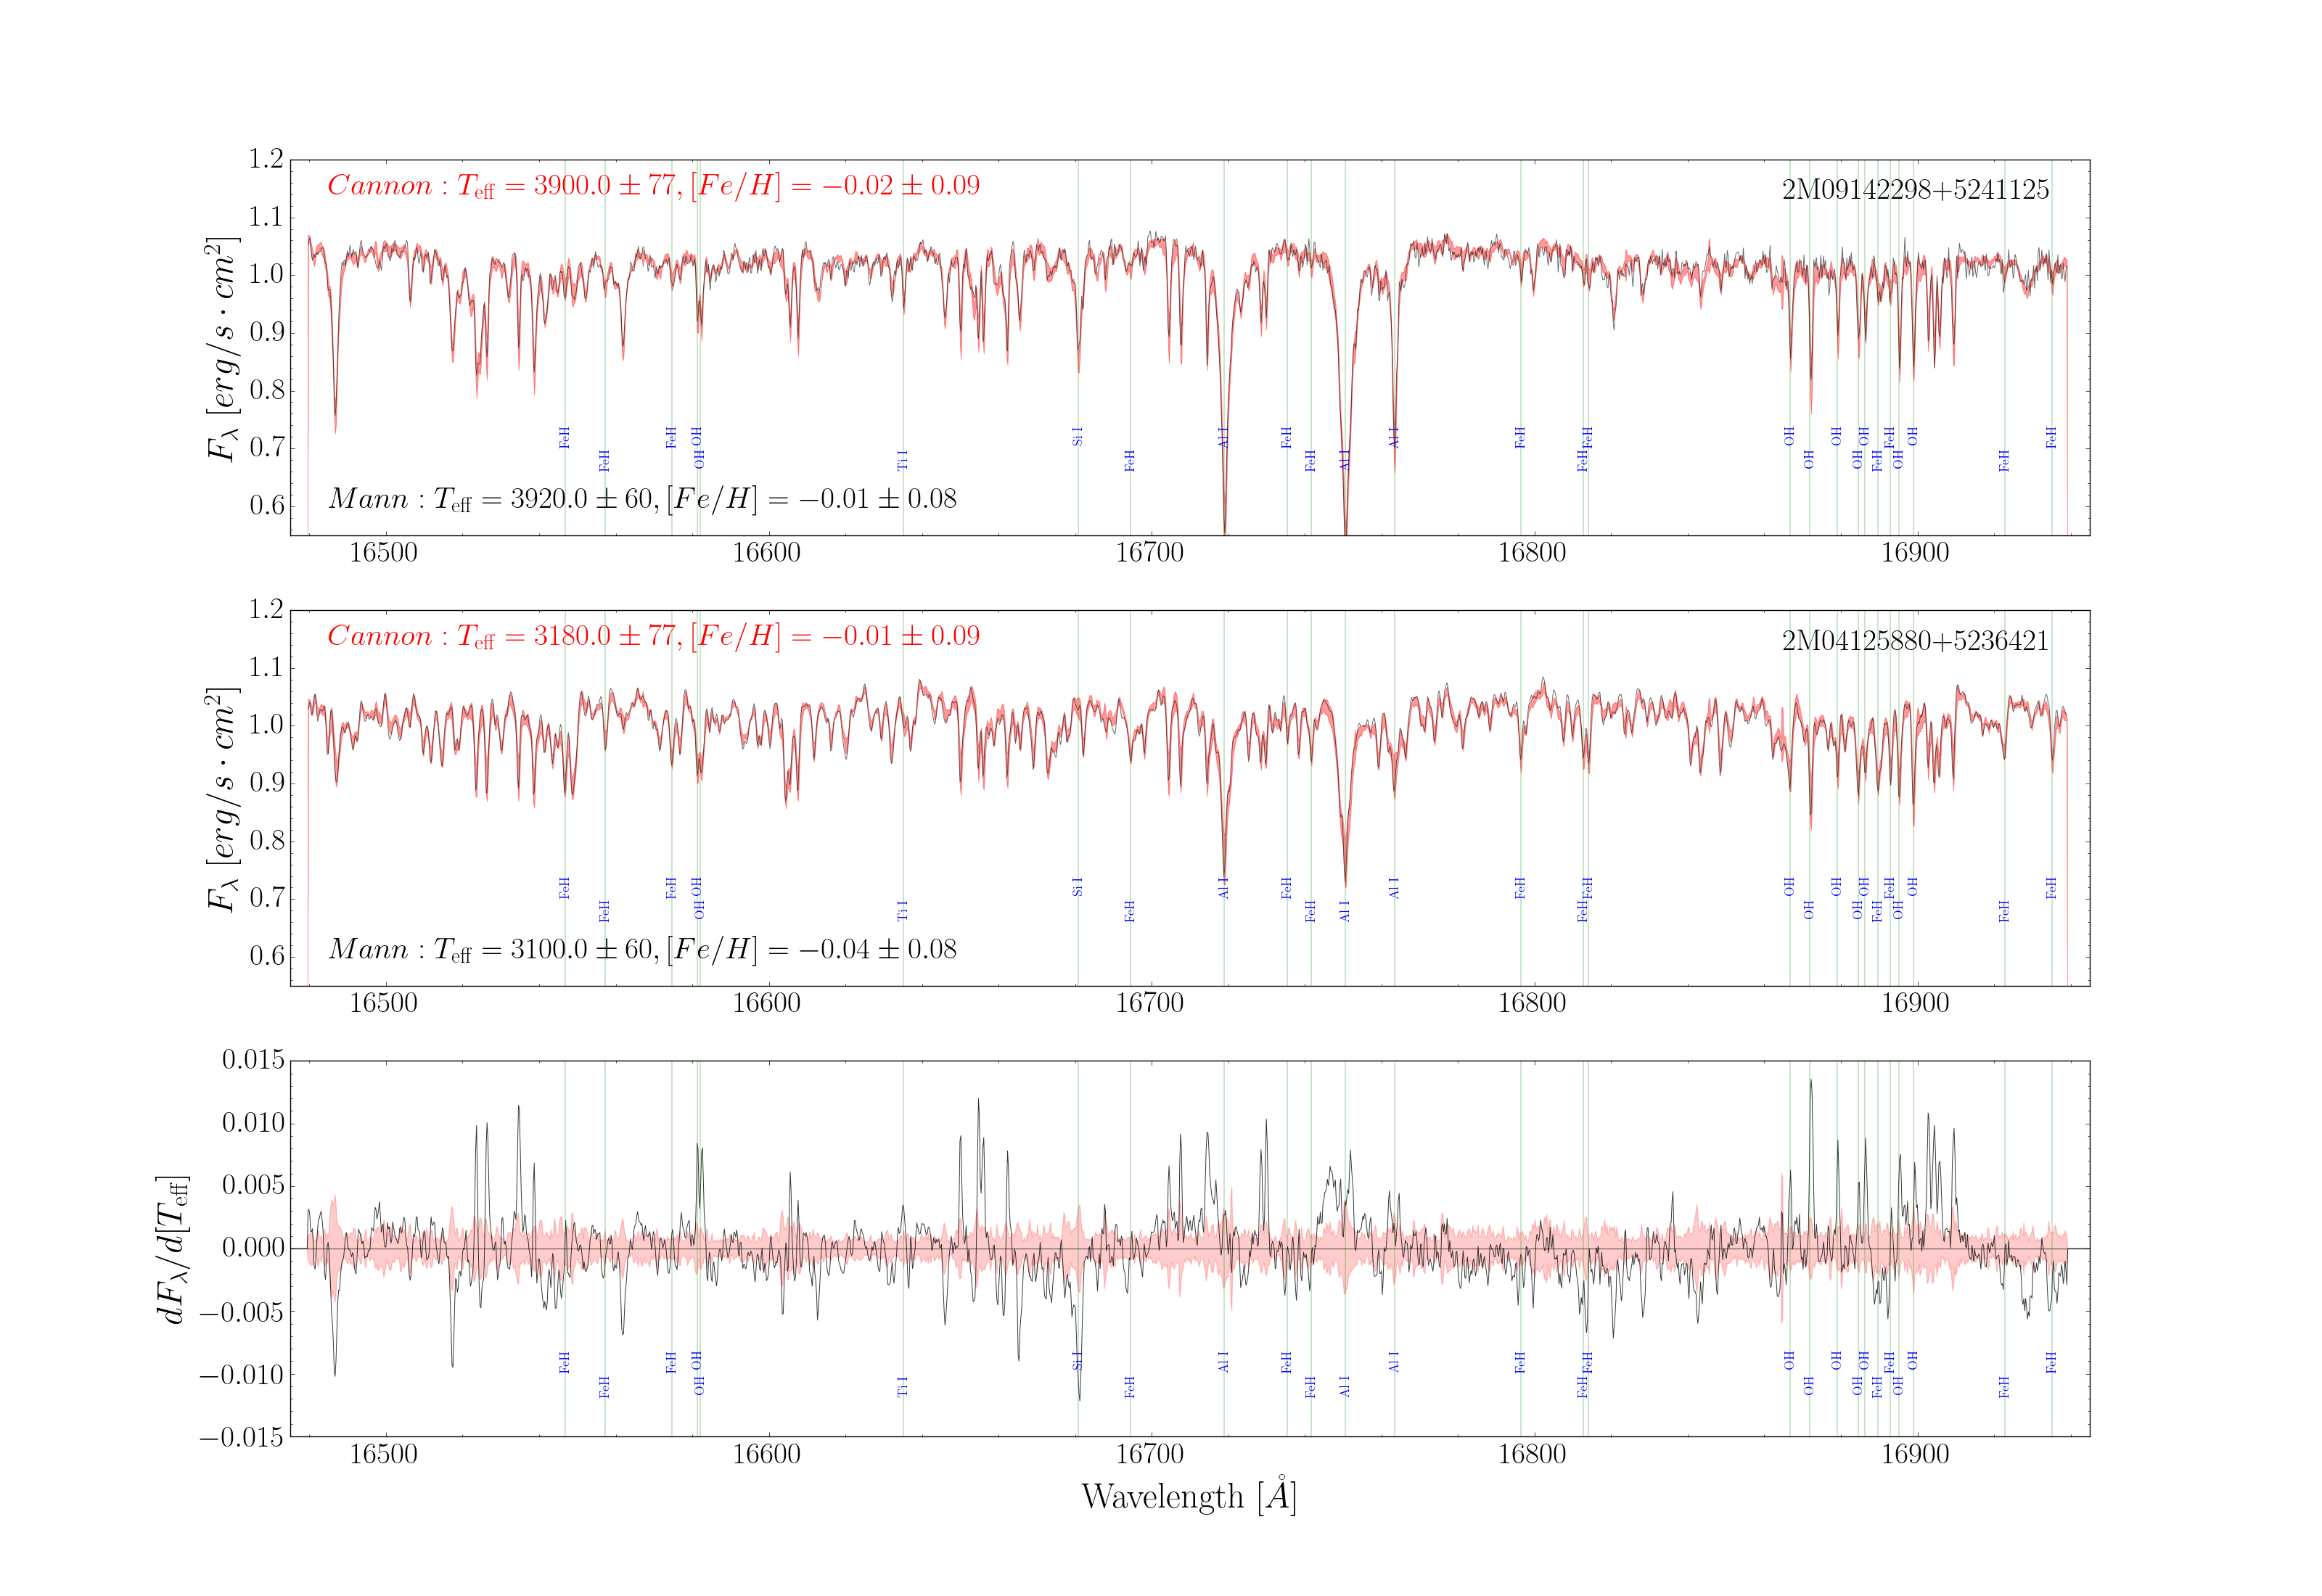
\includegraphics[width=16cm]{figures/demo_derivatives_teff3.png}
\end{center}
\caption{\textit{Top two panels:} Mann-trained model for varying temperatures.} \label{fig:demo_teff}
\end{figure}

\begin{figure}[ht]
\begin{center}
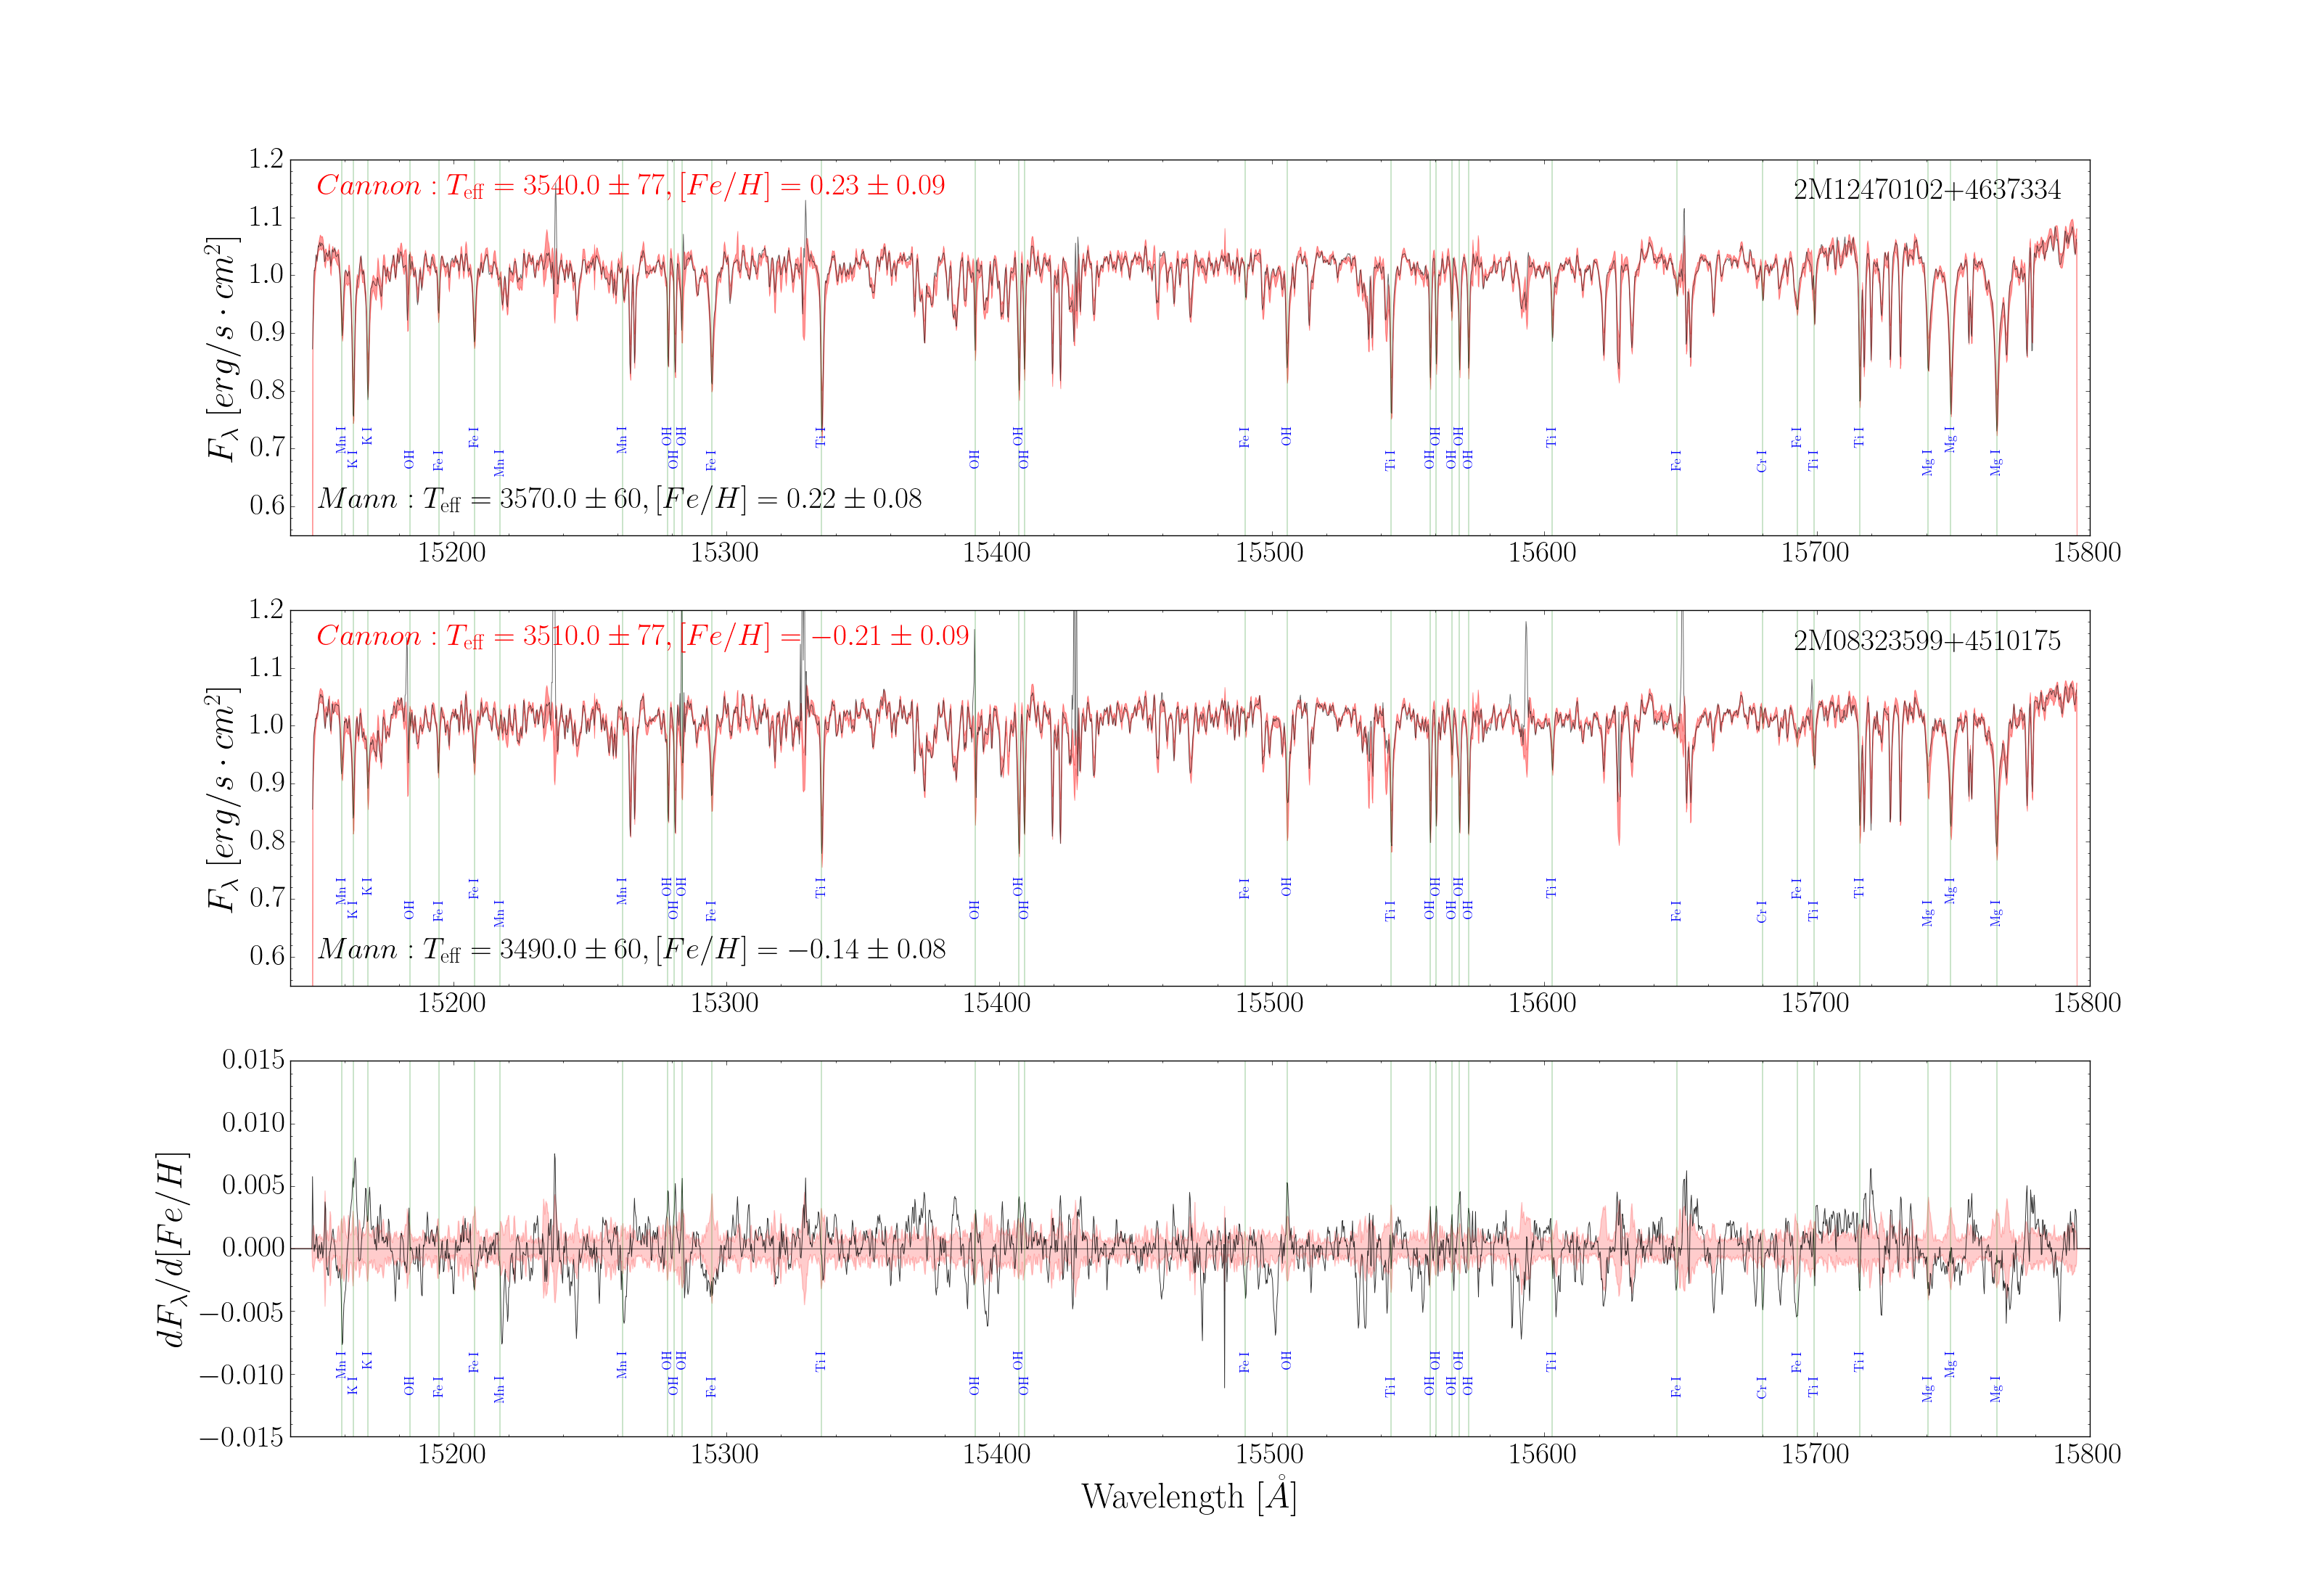
\includegraphics[width=16cm]{figures/demo_derivatives_feh1.png}
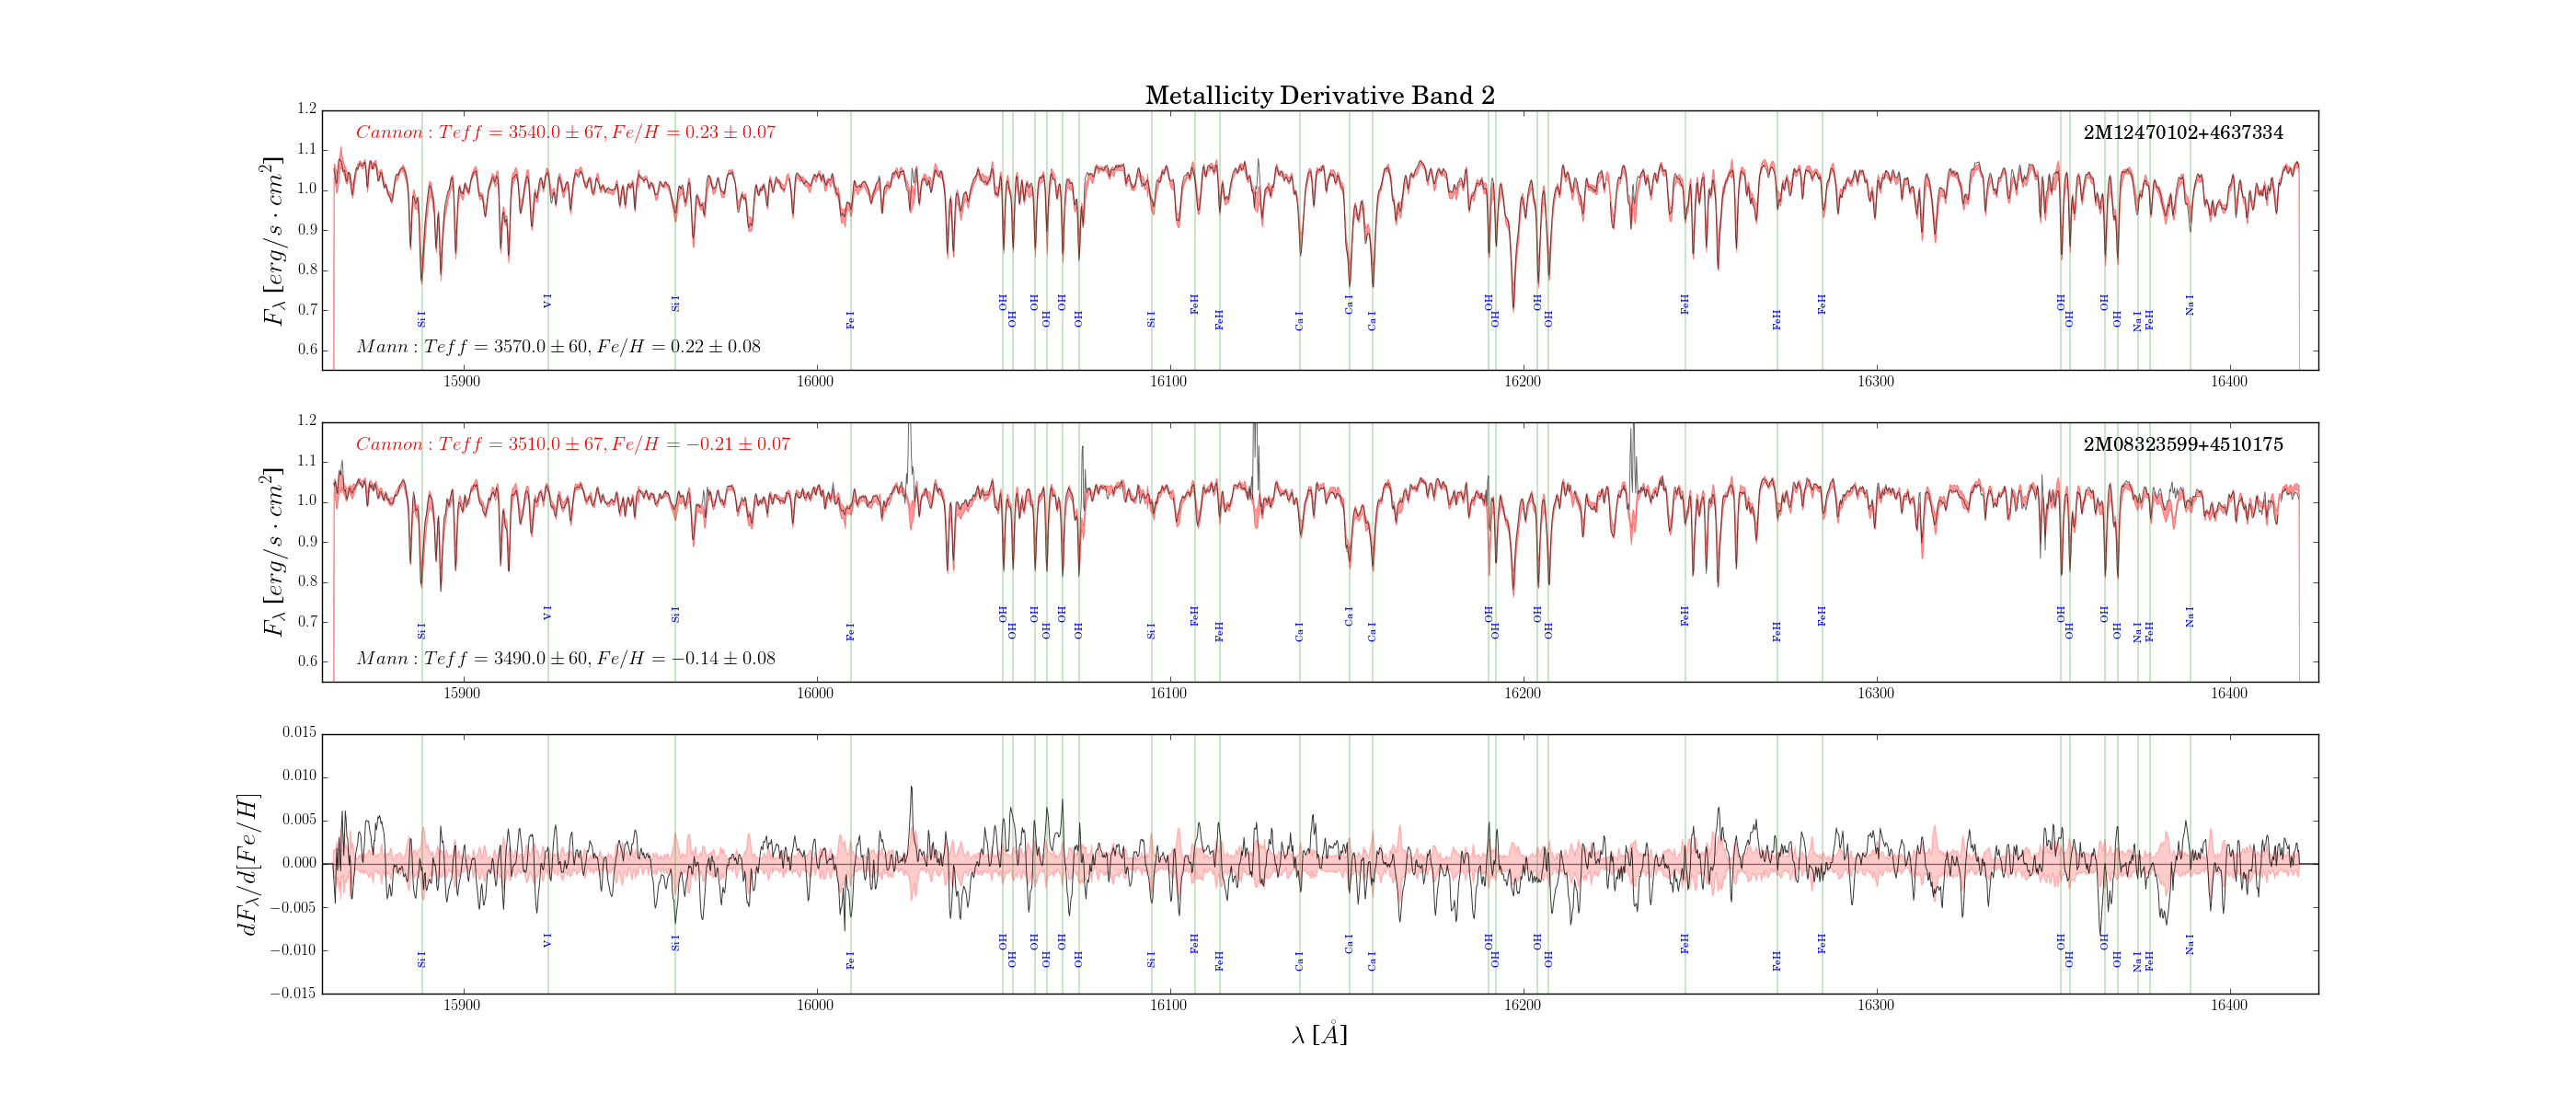
\includegraphics[width=16cm]{figures/demo_derivatives_feh2.png}
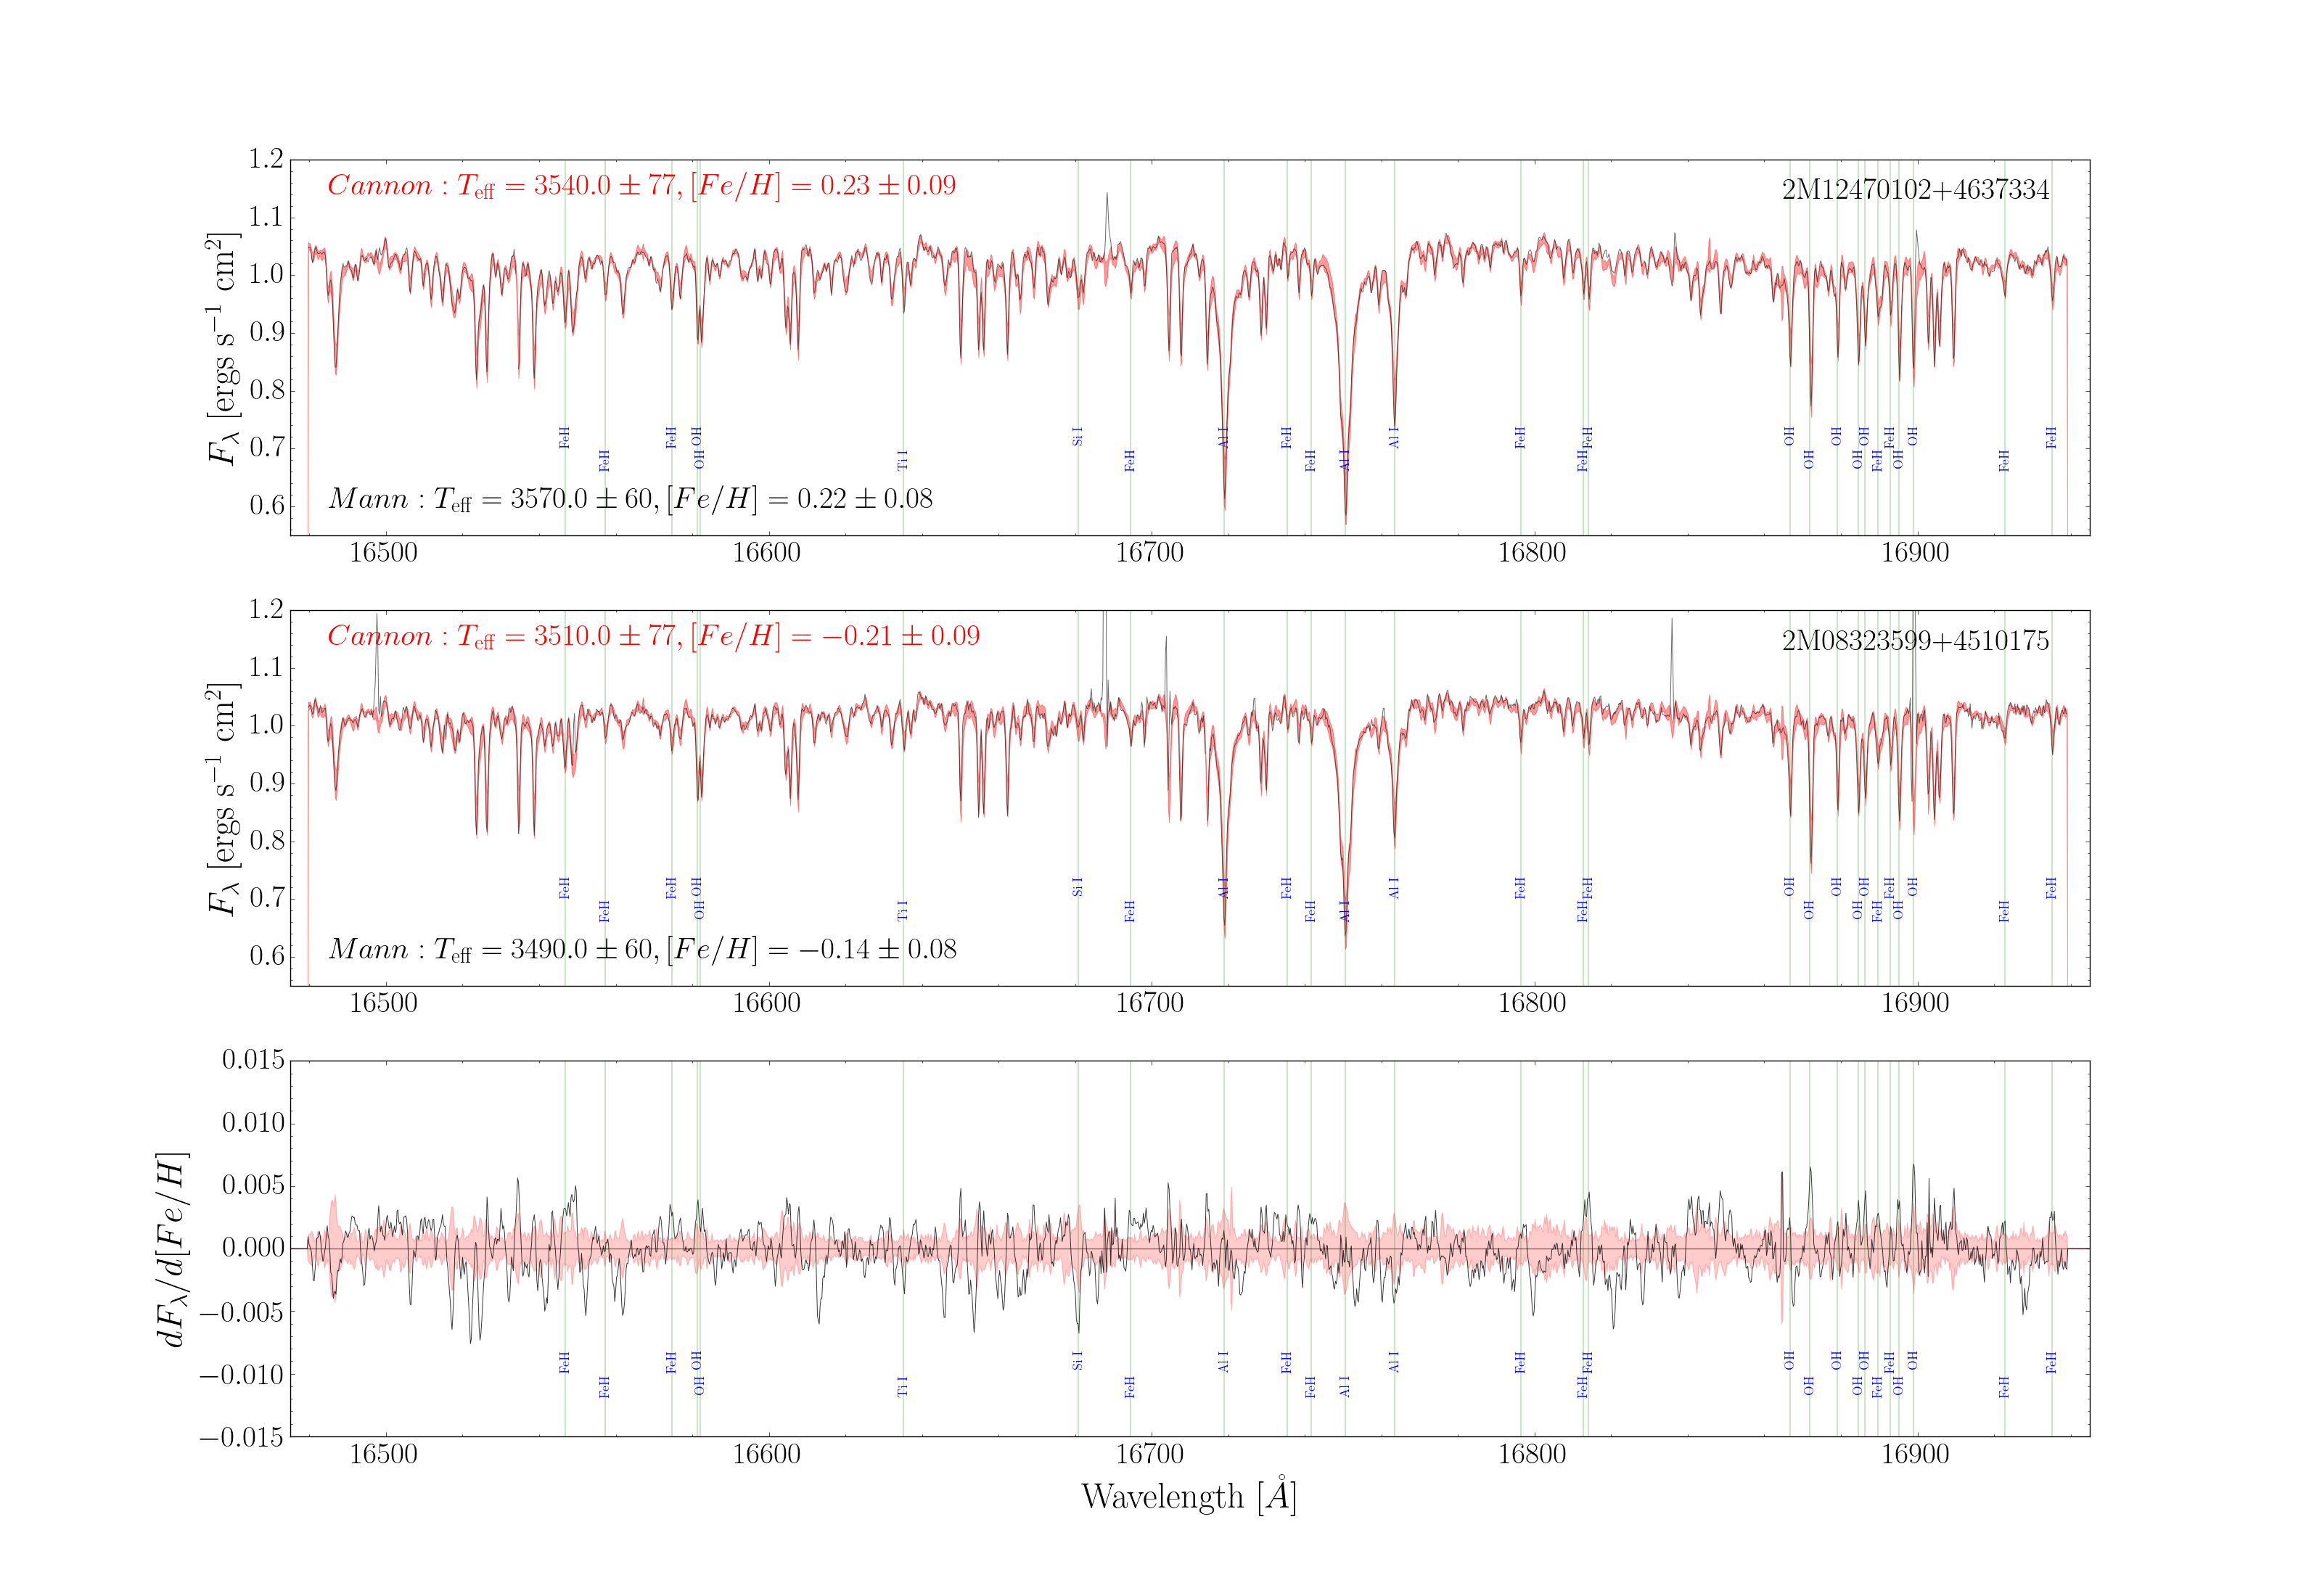
\includegraphics[width=16cm]{figures/demo_derivatives_feh3.png}
\end{center}
\caption{\textit{Top two panels:} Mann-trained model for varying metallicities.} \label{fig:demo_feh}
\end{figure}

\begin{figure}[ht]
\begin{center}
\includegraphics[width=12cm]{figures/west_spt_derivative.png}
\end{center}
\caption{Derivative plots for spectral type model.} \label{fig:west_derivative}
\end{figure}

\begin{figure}[ht]
\begin{center}
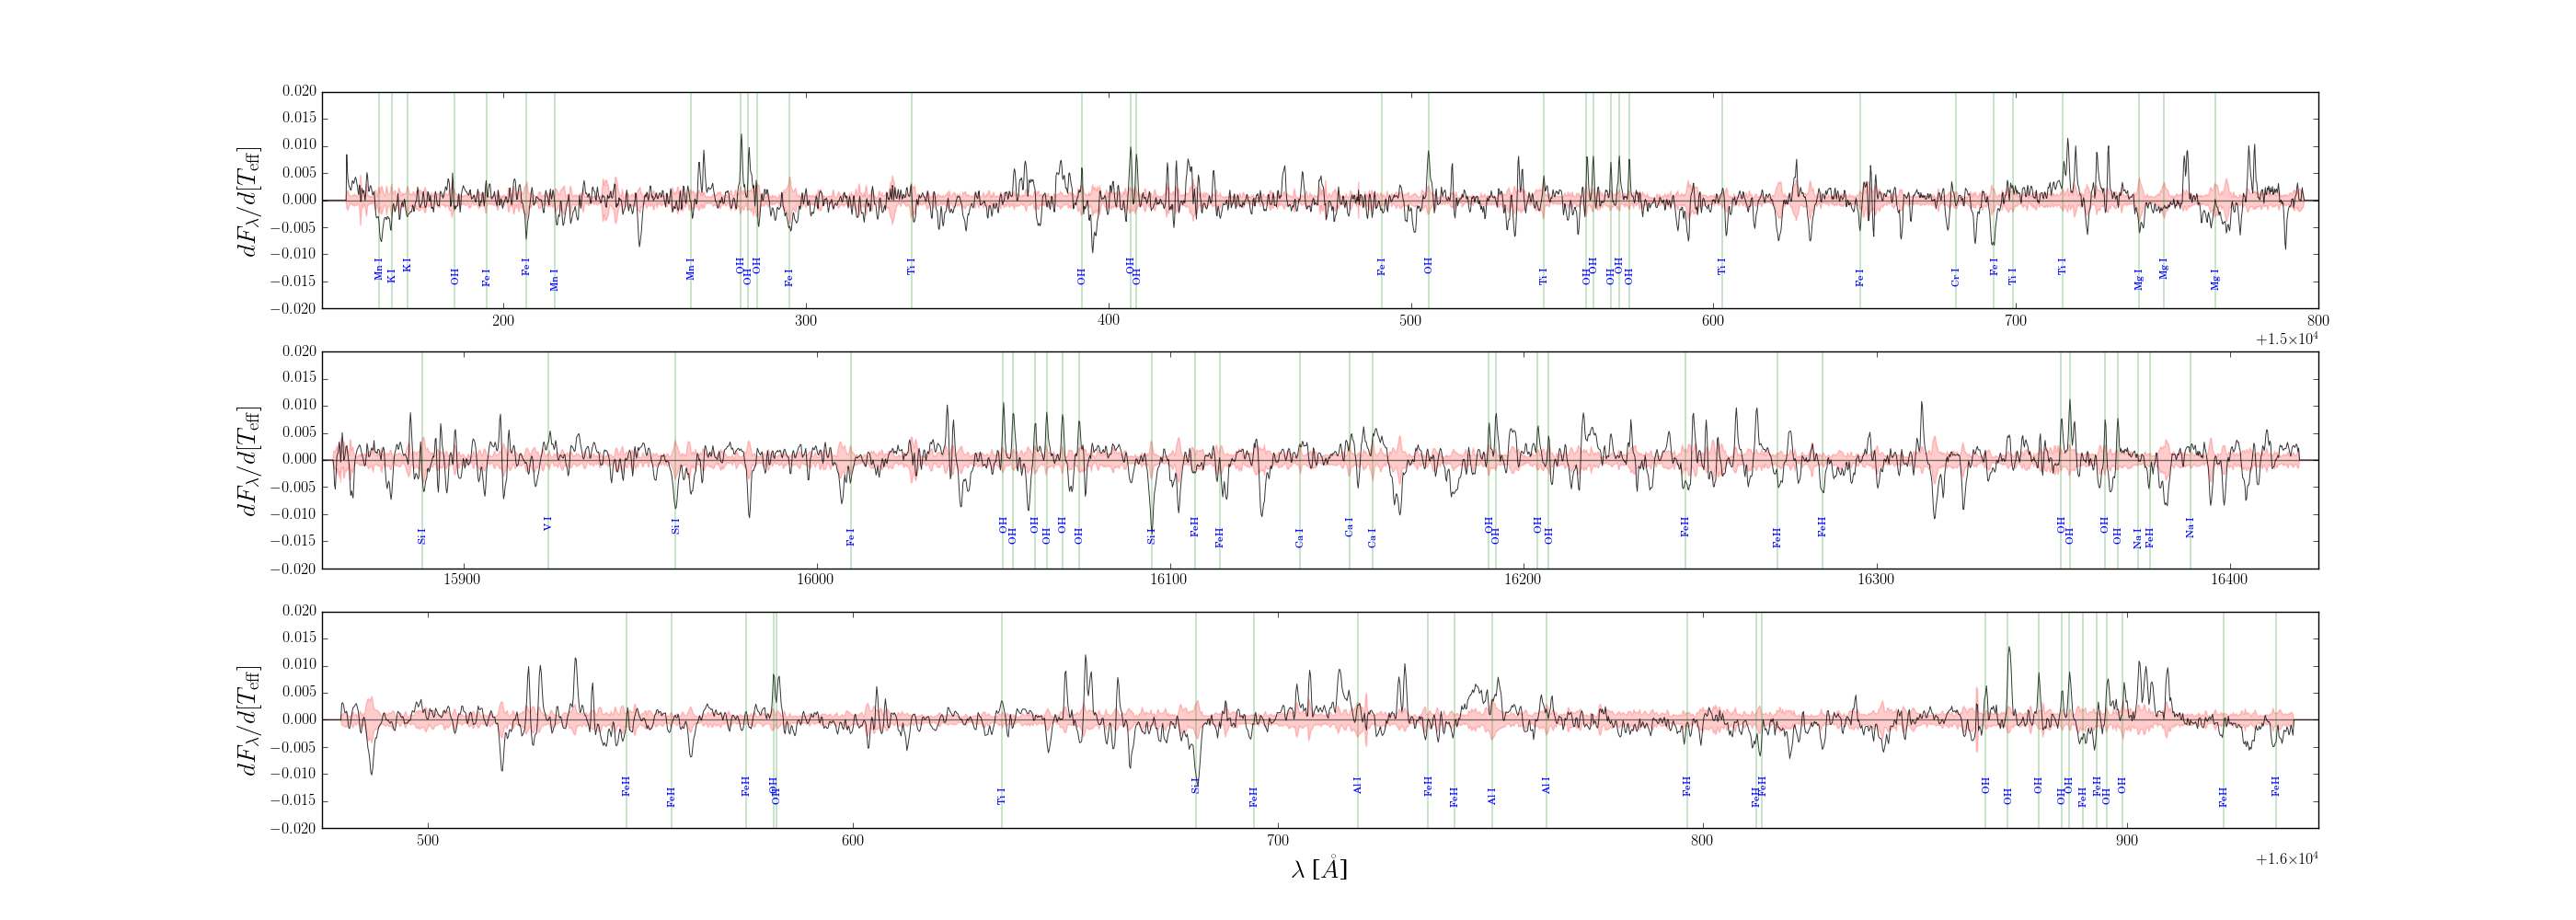
\includegraphics[width=15cm]{figures/derivative_jackknife_teff.png}
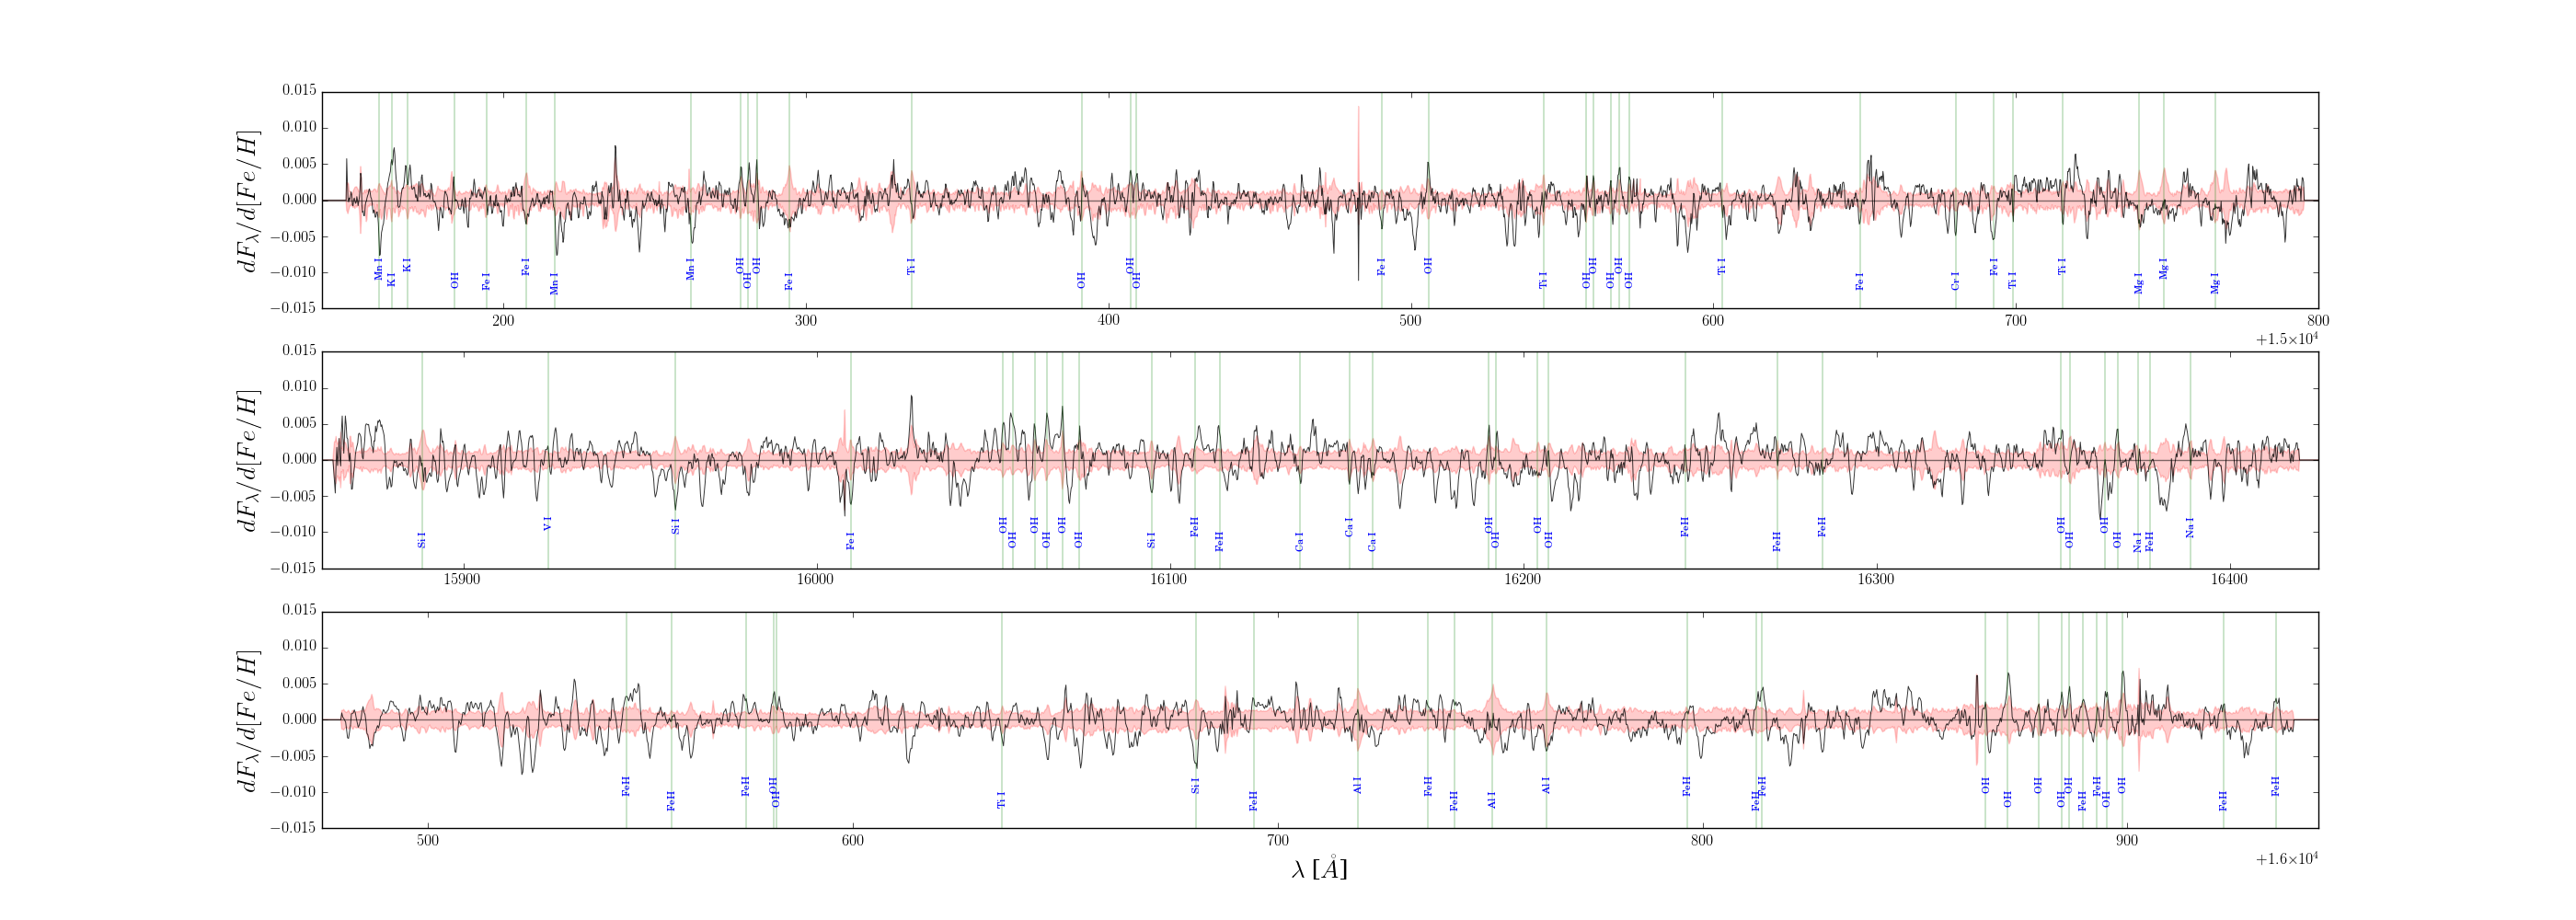
\includegraphics[width=15cm]{figures/derivative_jackknife_feh.png}
\end{center}
\caption{Derivative plots for physical parameter model. \textit{Top:} Derivative of flux with repsect to temperature. \textit{Bottom:} Derivative of flux with repsect to metallicity.} \label{fig:mann_derivative}
\end{figure}

%%==========================================================================================
\clearpage
\bibliographystyle{aasjournal}
\bibliography{ref}

\end{document}


